% !TEX root=../../mt-motion-analysis.tex
\chapter{Related work - Human Pose Estimation} \label{sec:pose_estimation}
\gls{hpe} is a well explored problem which, like many other computer vision tasks has developed rapidly in the recent years. The reasons behind this progress can mainly be explained by two factors. Firstly the emergence of computing power discussed in Section \ref{sec:dl-history}, allowing more expressive deep learning models. Secondly several datasets with images labeled with human body joints has been made available \cite{Chen2020}. These datasets not only provide data, but also introduces competition in the research community making it possible to compare the results of different approaches.

\section{Datasets} \label{sec:datasets}
%Some of the widely used datasets today are \gls{mpii} \cite{Andriluka2014}, \gls{coco} \cite{Lin2014}, \gls{aic-hkd} \cite{Wu2017}, and \gls{coco}-wholebody .% The two COCO datasets will now be described in more detail.

In this work models trained on the \gls{coco} dataset are used. \gls{coco} consists of 328k images containing 91 different object types. The images come from Google, Bing, and Flickr image search and are mainly hand annotated through Amazon Mechanical Turk. The interesting part of the dataset for this work is the one with human poses. In total there are 250k instances of people labeled with joint locations \cite{Lin2014}. The joints, 17 per person, in the dataset can be seen in Figure \ref{fig:coco}. Along with the datasets containing body keypoints mentioned above there are also datasets with dense keypoints for specific bodyparts, e.g. OneHand10k \cite{Wang2019}. \gls{coco}-wholebody \cite{Jin2020} is an attempt to combine these two types of datasets by extending \gls{coco} with dense keypoints at hands, feet, and faces. The resulting 133 joints can be seen in Figure \ref{fig:coco-wholebody}.

\begin{figure}
 \centering
 \begin{subfigure}[t]{0.4\textwidth}
   \centering
  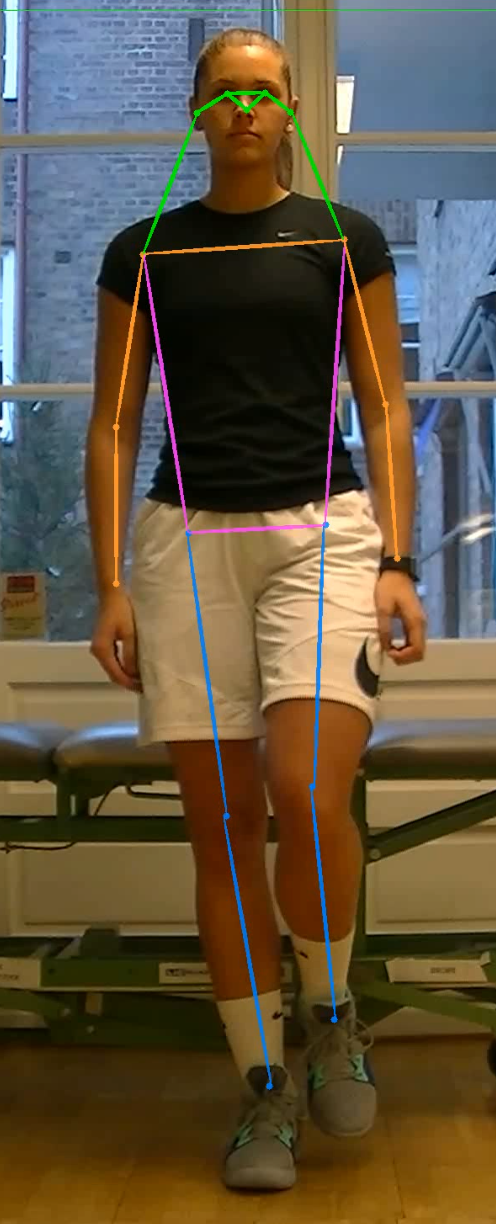
\includegraphics[width=0.6\textwidth]{files/figs/coco.png}
  \caption{Regular \gls{coco}.}
  \label{fig:coco}
 \end{subfigure}
 ~
 \begin{subfigure}[t]{0.4\textwidth}
   \centering
  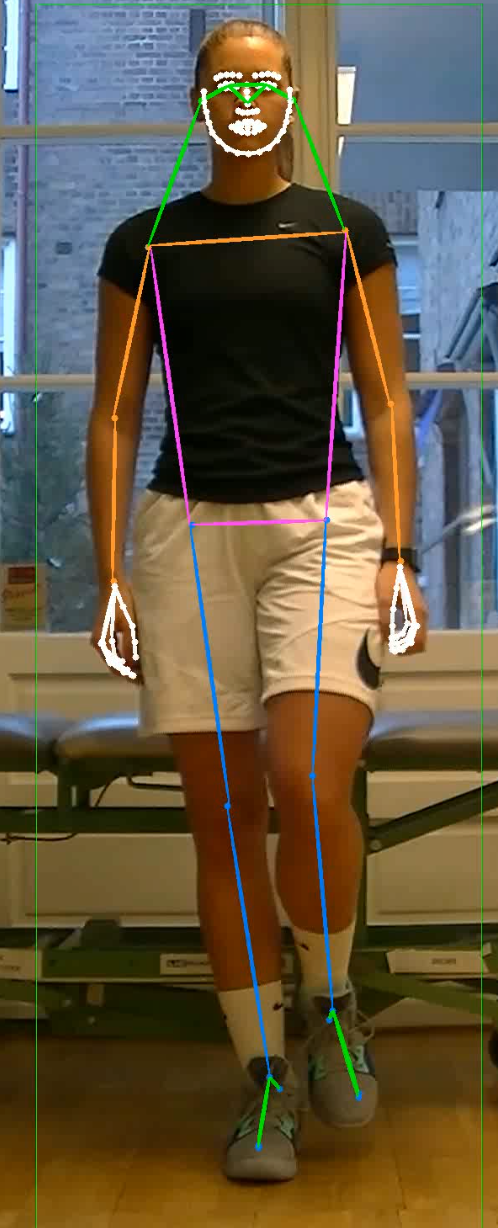
\includegraphics[width=0.6\textwidth]{files/figs/coco-wholebody.png}
  \caption{\gls{coco}-wholebody.}
  \label{fig:coco-wholebody}
 \end{subfigure}
 \caption{Keypoints for the two COCO datasets.}
\end{figure}

% \section{Pose estimation models}
\section{Background - Human pose estimation}
The \gls{hpe} problem has been explored since long before the most recent deep learning era. Pictoral Structures were introduced by Fishler and Elschlager in the 1970s. This meant identifying individual parts or features in images modeled with pair-wise spring-like connections \cite{Fischler1973}. After the progress of deep learning mentioned in Section \ref{sec:dl-history} Toshev and Szegedy \cite{Toshev2014} presented DeepPose, the first \gls{hpe} method based on \glspl{dnn}, in 2014. Today's \gls{hpe} methods are generally categorized as top-down or bottom-up approaches. This has to do with how they handle multiple persons. Bottom-up models starts by finding all keypoints for all persons in an image and then match them together to form persons. Top-down models on the other hand starts by finding bounding boxes for all individuals and then identifies keypoints for one person at a time. The sequential nature of the top-down methods and the fact that two models are needed means that bottom-up models scale better with the number of persons to analyze. However top-down models tends to be more accurate \cite{Cheng2019}.
% Since the application we present requires single person recognition only the top-down \gls{sota} methods presented below are used.

\section{Pose estimation models}
Below the \gls{hpe} models used in our work are presented. As we are interested in single person recognition the model used is of top-down type.

\subsection{High-Resolution Net (HRNet)} \label{sec:hrnet}
Sun et al. presented the \gls{hrnet} \cite{Sun2019} architecture in 2019, initially for \gls{hpe}, but also for other computer vision tasks such as semantic segmentation and object detection. Such problems had traditionally been solved using networks built on high-to-low resolution convolutions with increasing numbers of feature maps (e.g ResNet \cite{He2016}, VGGNet \cite{Simonyan2015}). The classification task was solved in the low-resolution space and then transformed back to form the high-resolution representation needed for e.g. the \gls{hpe}. Sun et al's proposed architecture preserves a high resolution representation throughout the network. It does so while also producing low-resolution/high dimensional representations suitable for classification.

The network architecture is shown in Figure \ref{fig:hrnet} and consists of four stages (blue blocks in depth direction in Figure) with convolutional layers. After each stage a new low-resolution representation is created by performing strided convolutions. At these instances the existing representations also exchange information by either nearest neighbor upsampling or strided convolutions. The $K$ estimated keypoints are represented as heatmaps, $\{\mathbf{H}_1, \hdots, \mathbf{H}_K\}$, indicating the locations. These heatmaps are formed from the last high-resolution feature map (top right in Figure \ref{fig:hrnet}). Corresponding ground truth heatmaps are generated by applying 2D Gaussians to the correct keypoint locations and the model is trained by minimizing the mean squared error between these \cite{Sun2019}. Although a high resolution heatmap is desirable as it gives smaller quantization errors, the computational cost increases quadratically with the size \cite{Zhang2020}. Hence, the performance of the model can be improved by extracting the region of interest from the input image. This can for instance be done using an object detection model trained to find humans.

Object detectors usually work by first producing a large number of regions of interest in the image which are then classified to either belong to some object class or the background. Faster R-CNN by Ren et al. \cite{Ren2017} is an example of such a detector where these steps are performed by a single \gls{cnn}. The model outputs bounding boxes and class scores for the objects in the image deemed not to be part of the background. %kanske skriva ngt om vad den ska blivit tr'nad p[?

%Hence, to make the computations feasible the input image is downsampled through strided convolutions, resulting in a four times smaller heatmap \cite{Wang2020}. To achieve more accurate results   %The heatmaps used for training are generated by applying 2D Gaussians to the dataset keypoints.

\begin{figure}
 \centering
 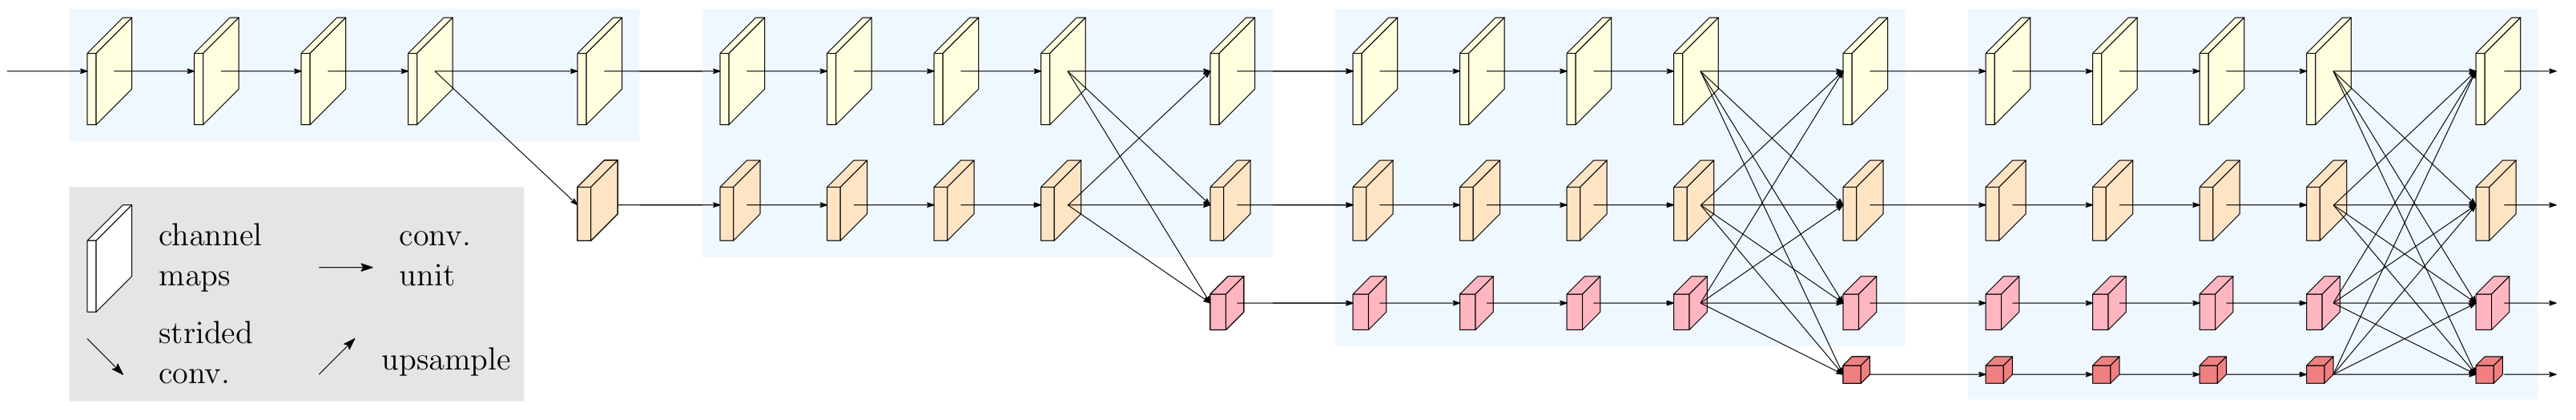
\includegraphics[width=\textwidth]{files/figs/hrnet.png}
 \caption{Network architecture for HRNet. The top row shows high resolution representations with fewer number of feature maps. Each step downwards reduces the resolution with a factor of two while the number of feature maps are doubled \cite{Wang2020}.}
 \label{fig:hrnet}
\end{figure}

% \FloatBarrier

\subsection{Distribution-Aware coordinate Representation of Key-point (DARK)} \label{sec:dark}
As discussed above a high resolution heatmap should result in higher accuracy, but is computationally expensive. Zhang et al. propose a method they call \gls{dark} \cite{Zhang2020} to reduce the quantization error by i) analyzing the distributions of the predicted heatmaps, and ii) creating the training heatmaps in a slightly new fashion.

The actual keypoint location is found at the maximal activation of the heatmap. Since it is smaller than the actual image this turns into a sub-pixel localisation problem. Newel et al. \cite{Newell2016} empirically found that a weighted average between the two highest activations, according to \eqref{eq:pixel-empiric}, yielded a good result.

\begin{equation}
  \pmb{p} = \symbfit{m} + \frac{1}{4}\frac{\symbfit{s} - \symbfit{m}}{\lVert \symbfit{s} - \symbfit{m} \rVert_2}
  \label{eq:pixel-empiric}
\end{equation}
\begin{conditions}
    \italbf{p}   & =   & predicted maximum \\
    \italbf{m}      & =   & highest activation \\
    \italbf{s}      & =   & second highest activation
\end{conditions}

This has been the de facto standard heatmap decoding, but Zhang et al. suggests using the fact that the heatmaps used for training usually are created as 2D Gaussian distributions, i.e. that the heatmaps can be expressed as \eqref{eq:gaussian-heatmap}.

\begin{equation}
  \mathcal{G}(\pmb{x}; \pmb{\mu}, \Sigma) = \frac{1}{2\pi \mid \Sigma \mid^{\frac{1}{2}}}
  \exp \Big( -\frac{1}{2} (\pmb{x} - \pmb{\mu})^\intercal \Sigma^{-1} (\pmb{x} - \pmb{\mu}) \Big)
  \label{eq:gaussian-heatmap}
\end{equation}
\begin{conditions}
    $$\pmb{\mu}$$ & =   & maximum of heatmap \\
    \italbf{x}    & =   & pixel location \\
    $$\Sigma$$    & =   & diagonal covariance matrix
\end{conditions}

By Taylor expanding of the logarithm of \eqref{eq:gaussian-heatmap} in the point \italbf{m}, i.e. the point with the highest sampled activation, an expression for $\pmb{\mu}}$ is obtained:

\begin{equation}
    \pmb{\mu} = \pmb{m} - \Big(\mathcal{D''}(\pmb{m})\Big)^{-1} \mathcal{D'}(\pmb{m})
    \label{eq:opt-mu}
\end{equation}
\begin{conditions}
    $$\mathcal{D}(\pmb{x})$$ & = & $-\frac{1}{2} (\pmb{x} - \pmb{\mu})^\intercal \Sigma^{-1} (\pmb{x} - \pmb{\mu})$, \\
      & & i.e. the non constant term in the logarithm of $$\mathcal{G}$$ \eqref{eq:gaussian-heatmap}
\end{conditions}

The derivatives $\mathcal{D'}(\pmb{m})$ and $\mathcal{D''}(\pmb{m})$ are efficiently estimated from the heatmap. As this approach strongly assumes a Gaussian structure it is proposed to modulate the heatmap before estimating the maximal activation. This is done by performing a convolution with a Gaussian kernel with the same covariance as the one used for the training data.

The second improvement suggested by Zhang et al. concerns the creation of the training heatmaps. Traditionally these have been created from the quantized keypoint locations, resulting in a slightly biased heatmap. In Figure \ref{fig:pixel-quantization} this would correspond to having the peak activation in the purple dot. By instead using the non-quantized location an unbiased heatmap is obtained. This would correspond to having the peak off-grid, in the blue dot in Figure \ref{fig:pixel-quantization}.

\begin{figure}
  \centering
  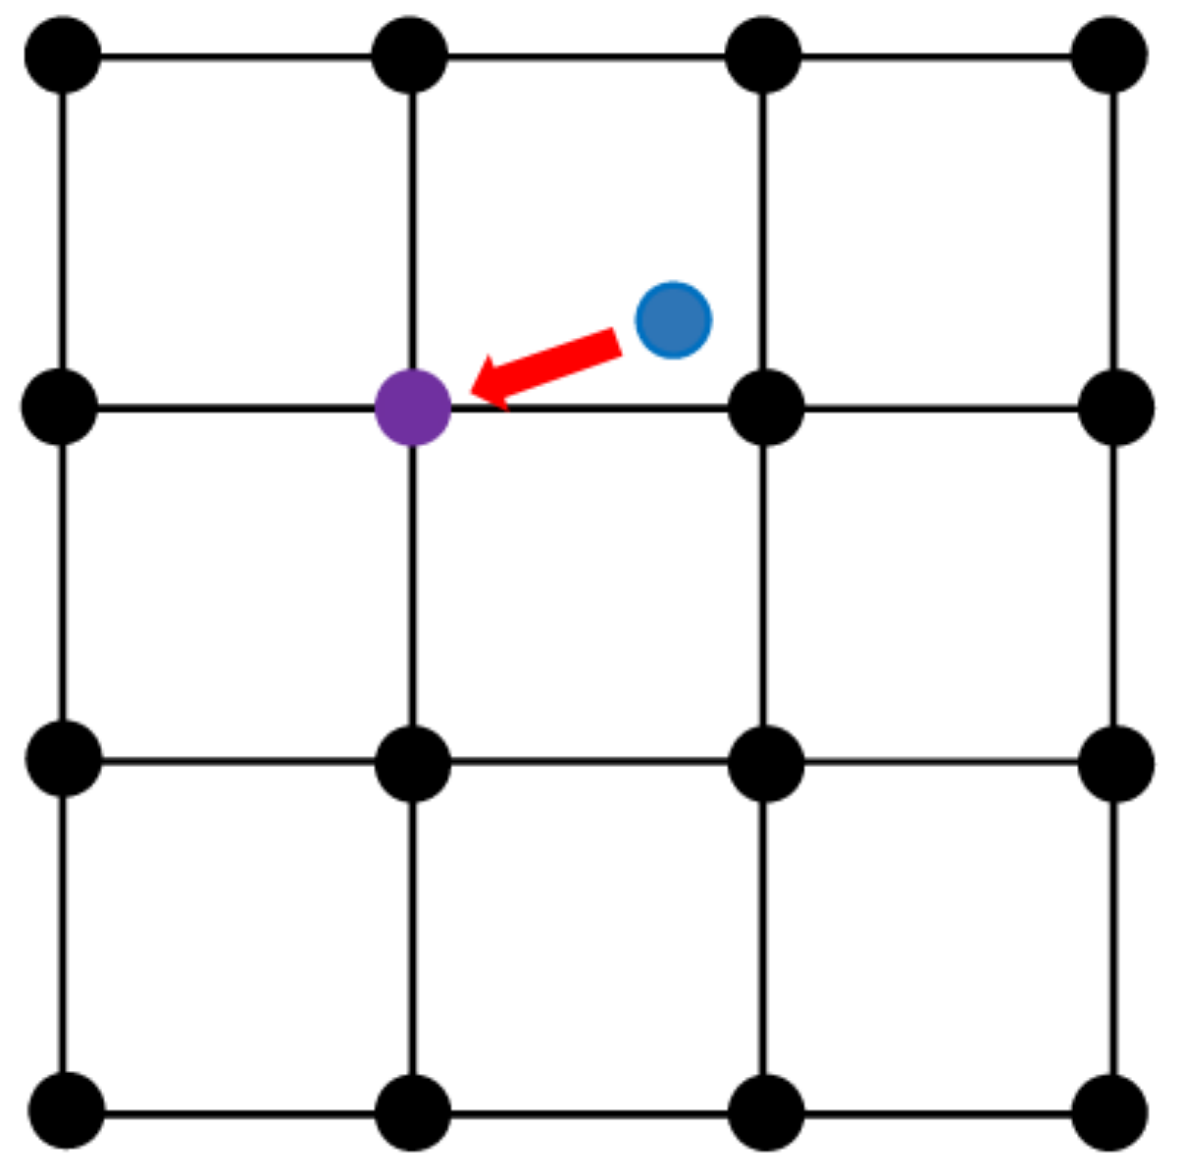
\includegraphics[width=0.4\textwidth]{files/figs/quantization.png}
  \caption{Quantization error due to off-grid keypoint location. Correct location (blue) represented by on-grid coordinate, here using floor quantization \cite{Zhang2020}. SKRIV ANTAGLIGEN NAGOT BATTRE HAR!!!!!}
  \label{fig:pixel-quantization}
\end{figure}

% \FloatBarrier

% The combination of DARK and HRNet is the method that as of today yields the highest accuracy on both the COCO and MPII dataset
